\section{Experiments}\label{experiments}
%
\subsection{Shrinking the gap on in-context learning}\label{eval_ker}
%
We begin by empirically motivating the ${\sf Hyena}$ design, including the choice of long convolution parametrization. We consider the suite of tasks described in Table \ref{table:grok}.
%
\begin{table}[b]
    \small
    \centering
    \caption{A selection of our \textit{mechanistic design} benchmarks.}
    \setlength{\tabcolsep}{5.8pt}
    \label{table:grok}
    \begin{tabular}{@{}c|cc@{}}
    \toprule
    \textbf{Task} &\multicolumn{1}{c}{\textbf{Prompt}}&\multicolumn{1}{c}{\textbf{Target}}\\
    \midrule 
    Associative Recall & a, $1$, b, e, $3$, f, b & e\\  
    Majority & a, g, g, g, e, f, g & g \\
    Counting & a, b, b, b, a, c, b & 4\\
    ICL of Functions & $x_0$, $f(x_0)$, $\dots x_n$ & $f(x_n)$ \\ 
    Arithmetic & $1$, $3$, $5$, $+$, $6$, $8$, $3$ & $8$, $1$, $8$ \\
    \bottomrule
    \end{tabular}
\end{table}
%
\begin{figure*}[t]
  \centering
  \begin{tikzpicture}[font=\small]

\definecolor{coral25314160}{RGB}{253,141,60}
\definecolor{cornflowerblue107174214}{RGB}{107,174,214}
\definecolor{darkgray176}{RGB}{176,176,176}
\definecolor{lightgray204}{RGB}{204,204,204}
\definecolor{lightsteelblue158202225}{RGB}{158,202,225}
\definecolor{orangered2308513}{RGB}{230,85,13}
\definecolor{powderblue198219239}{RGB}{198,219,239}
\definecolor{steelblue49130189}{RGB}{49,130,189}
\definecolor{brown}{RGB}{165,42,42}
\definecolor{cornflowerblue}{RGB}{100,149,237}
\definecolor{darkgray176}{RGB}{176,176,176}
\definecolor{indianred}{RGB}{205,92,92}
\definecolor{lightgray204}{RGB}{204,204,204}
\definecolor{teal}{RGB}{0,128,128}
\definecolor{lightseagreen}{RGB}{32,178,170}

\begin{groupplot}[group style={group size=4 by 1, horizontal sep=.8cm}]
\nextgroupplot[
width=.28\linewidth,
xlabel={$\sf Sequence Length$}, 
title={$\sf Vocabulary~Size$:~$10$}, title style={at={(.5,.92)}},
xlabel={$\sf Sequence~Length$}, xlabel style={at={(.5,-.15)}},
xmin=0, xmax=4,
ymin=0, ymax=100,
xtick={0,1,2,3,4}, xticklabels={$2^7$,$2^9$,$2^{11}$,$2^{13}$,$2^{15}$},
ytick={0,20,40,60,80,100}, yticklabels={0,20,40,60,80,100},
grid=both,
%ymode=log,
]
\addplot [line width=1pt, cornflowerblue107174214, dashed, mark=diamond*, mark size=3, mark options={solid}]
table {%
0 100
1 100
2 100
3 100
4 100
};
\addplot [line width=1pt, lightsteelblue158202225, dotted, mark=*, mark size=3, mark options={solid}]
table {%
0 98
1 99.8
2 99.4
3 99.4
4 98.8
};
\addplot [line width=1pt, powderblue198219239, mark=triangle*, mark size=3, mark options={solid,rotate=180}]
table {%
0 97.8
1 99.4
2 98.4
3 99.4
4 99.2
};
\addplot [line width=1pt, lightseagreen, mark=triangle*, mark size=3, mark options={solid}]
table {%
0 85.4
1 93
2 91.8
3 93.6
4 97.6
};
\addplot [line width=1pt, teal, mark=star, mark size=3, mark options={solid}]
table {%
0 62.6
1 98
2 97.2
3 50.4
4 56.8
};
\addplot [line width=1pt, indianred, mark=mystar, mark size=3, mark options={solid}]
table {%
0 93
1 99
2 99.6
3 100
4 100
};

\nextgroupplot[
width=.28\linewidth, 
title={$\sf Vocabulary~Size$:~$20$}, title style={at={(.5,.92)}},
xlabel={$\sf Sequence~Length$}, xlabel style={at={(.5,-.15)}},
xmin=0, xmax=4,
ymin=0, ymax=100,
xtick={0,1,2,3,4}, xticklabels={$2^7$,$2^9$,$2^{11}$,$2^{13}$,$2^{15}$},
ytick={0,20,40,60,80,100}, yticklabels={},
grid=both,
]

\addplot [line width=1pt, cornflowerblue107174214, dashed, mark=diamond*, mark size=3, mark options={solid}]
table {%
0 91
1 98
2 99.4
3 99.8
4 100
};
\addplot [line width=1pt, lightsteelblue158202225, dotted, mark=*, mark size=3, mark options={solid}]
table {%
0 71.6
1 88.8
2 93.9
3 97
4 94
};
\addplot [line width=1pt, powderblue198219239, mark=triangle*, mark size=3, mark options={solid,rotate=180}]
table {%
0 71.5
1 84.4
2 92.8
3 93.6
4 91.4
};
\addplot [line width=1pt, lightseagreen, mark=triangle*, mark size=3, mark options={solid}]
table {%
0 20
1 65
2 59.8
3 39.6
4 26.2
};
\addplot [line width=1pt, teal, mark=star, mark size=3, mark options={solid}]
table {%
0 16.2
1 18.2
2 35.2
3 16.4
4 15.8
};
\addplot [line width=1pt, indianred, mark=mystar, mark size=3, mark options={solid}]
table {%
0 93
1 99
2 99.6
3 100
4 100
};

\nextgroupplot[
width=.28\linewidth, 
title={$\sf Vocabulary~Size$:~$30$}, title style={at={(.5,.92)}},
xlabel={$\sf Sequence~Length$}, xlabel style={at={(.5,-.15)}},
xmin=0, xmax=4,
ymin=0, ymax=100,
xtick={0,1,2,3,4}, xticklabels={$2^7$,$2^9$,$2^{11}$,$2^{13}$,$2^{15}$},
ytick={0,20,40,60,80,100}, yticklabels={},
grid=both,
]
\addplot [line width=1pt, cornflowerblue107174214, dashed, mark=diamond*, mark size=3, mark options={solid}]
table {%
0 25.7
1 85
2 93.1
3 91.2
4 95.2
};
\addplot [line width=1pt, lightsteelblue158202225, dotted, mark=*, mark size=3, mark options={solid}]
table {%
0 14.3
1 44.1
2 18.4
3 25.4
4 13.4
};
\addplot [line width=1pt, powderblue198219239, mark=triangle*, mark size=3, mark options={solid,rotate=180}]
table {%
0 13.2
1 23.2
2 28.1
3 16.7
4 8.4
};
\addplot [line width=1pt, lightseagreen, mark=triangle*, mark size=3, mark options={solid}]
table {%
0 12.7
1 21.6
2 12.7
3 15.2
4 11.4
};
\addplot [line width=1pt, teal, mark=star, mark size=3, mark options={solid}]
table {%
0 9.6
1 9.3
2 10.3
3 7.4
4 9.7
};
\addplot [line width=1pt, indianred, mark=mystar, mark size=3, mark options={solid}]
table {%
0 38.8
1 98
2 98.8
3 99.2
4 99.6
};

\nextgroupplot[
width=.28\linewidth, 
title={$\sf Vocabulary~Size$:~$40$}, title style={at={(.5,.92)}},
xlabel={$\sf Sequence~Length$}, xlabel style={at={(.5,-.15)}},
xmin=0, xmax=4,
ymin=0, ymax=100,
xtick={0,1,2,3,4}, xticklabels={$2^7$,$2^9$,$2^{11}$,$2^{13}$,$2^{15}$},
ytick={0,20,40,60,80,100}, yticklabels={},
grid=both,
legend style = {
    draw=black,
    fill=none,
     /tikz/column 6/.style={column sep=5pt,},
    at={(0.45,-.35)},
},
legend columns=6
]
\addplot [line width=1pt, indianred, mark=mystar, mark size=3, mark options={solid}]
table {%
0 12.4
1 66.5
2 99.1
3 100
4 100
};\addlegendentry{$\sf Hyena$};

\addplot [line width=1pt, cornflowerblue107174214, dashed, mark=diamond*, mark size=3, mark options={solid}]
table {%
0 20.4
1 38.6
2 52
3 51.2
4 49.7
};\addlegendentry{$\sf CKConv$};
\addplot [line width=1pt, lightsteelblue158202225, dotted, mark=*, mark size=3, mark options={solid}]
table {%
0 10
1 16.4
2 8.4
3 4.3
4 4.2
};\addlegendentry{$\sf Transfer~Function$};
\addplot [line width=1pt, powderblue198219239, mark=triangle*, mark size=3, mark options={solid,rotate=180}]
table {%
0 10.2
1 12.2
2 8.6
3 4.1
4 4
};\addlegendentry{$\sf H3$};
\addplot [line width=1pt, lightseagreen, mark=triangle*, mark size=3, mark options={solid}]
table {%
0 20
1 9.1
2 10.4
3 12
4 7.99
};\addlegendentry{$\sf Conv1D$};
\addplot [line width=1pt, teal, mark=star, mark size=3, ]
table {%
0 14.2
1 6.7
2 10.8
3 4.1
4 4.8
};\addlegendentry{$\sf FNO$};
\end{groupplot}

\draw ({$(current bounding box.south west)!0.5!(current bounding box.south east)$}|-{$(current bounding box.south west)!1.1!(current bounding box.north west)$}) node[
  scale=1.1,
  anchor=north,
  text=black,
  rotate=0.0
]{\textbf{Associative~Recall}};
\end{tikzpicture}

  \caption{Benchmark of long convolution parametrizations in order $2$ ${\sf Hyena}$ operators on associative recall (\%). Our results show that implicit parametrizations scale more favorably in vocabulary size (number of possible values of tokens in the input) and length of the sequence.}
  \label{fig:synthetics1}
\end{figure*}
%
Our evaluation is grounded in recent work on mechanistic interpretability of Transformers \citep{elhage2021mathematical,power2022grokking,olsson2022context,zhang2022unveiling}. Recently, associative recall, in particular, has been successfully used to guide the design of H3 \citep{dao2022hungry}. We extend the suite of tasks from these works and include benchmarking more challenging versions of each task . For example, solving associative recall with a vocabulary size of only $10$ reveals whether a model is structurally capable of performing recall. Testing on much longer sequences and larger vocabularies reveals additional gaps in performance that are otherwise hidden.
%
\paragraph{How to parametrize long convolutions}
%
We compare the performance of the following long convolution parametrizations for $S^1$ and $S^2$ in an order $2$ Hyena:
%
\begin{itemize}[leftmargin=0.1in]
    \item Conv1d: Explicit convolutions (regular convolution layers with fixed filter size).
    \item FNO: Filters parametrized explicitly in the frequency-domain \citep{li2020fourier}.
    \item H3: Implicit parametrization using state-space models (SSMs), in particular the standard S4 \citep{gu2021efficiently}. 
    \item TransferFunc: Implicit parametrization via transfer functions, a classical system-theoretic generalization of SSMs\footnote{Transfer functions roughly correspond to a frequency-domain representation of SSMs.} 
    \item CKConv: Implicit parametrization using {$\sf FFN$s} \citep{romero2021ckconv}. 
    \item ${\sf Hyena}$: Combination of implicit parametrizations via {$\sf FFN$s} (with exponential decay modulation as shown in Figure \ref{fig:modul}), and short explicit filters.
\end{itemize}
%
All models have the same width and $2$ layers. Figure \ref{fig:synthetics1} shows implicit approaches based on {\sf FFNs} outperform other long convolutions, with the gap widening on longer sequences and larger vocabulary sizes. We train a different model on each setting of sequence length and vocabulary size. The ranking is correlated with the ability to decouple sequence length from parameter count (${\sf Hyena}$, CKConv, TransferFunc, H3) and expressivity (Hyena, CKConv). We observe similar trends on the other tasks.
%
\paragraph{Pushing sequence length to the limit}
%
Next, we evaluate associative recall performance on extremely long sequences of length $131$k. To the best of our knowledge, these represent the first empirical display of attention-free in-context learning on sequences of this length. The gap between parametrization schemes widens as shown in Appendix A, with ${\sf Hyena}$ outperforming CKConv by $80$ points.
%
\paragraph{Comparing operators}
%
We repeat our associative recall experiment, this time benchmarking different $2$ layer models rather than changing the convolution parametrization: an order $2$ Hyena, GSS \citep{mehta2022long}, H3 \citep{dao2022hungry}, AFT-conv \citep{zhai2021attention}, RWKV \citep{PENG_RWKV-LM_2021}, and a standard GPT \citep{brown2020language} using FlashAttention \citep{dao2022flashattention}. As shown in Table \ref{table:synthetic2}, ${\sf Hyena}$ is the only operator able to solve the task. Our results challenge the observation that only Transformers are capable of challenging in-context learning.
%
\begin{table}[t]
\small
\centering
\caption{Test accuracy (\%) for associative recall on longer sequences, vocabulary size $30$. The symbol \xmark~is used to mark settings where the model does not fit in memory.}
\label{table:synthetic2}
\setlength{\tabcolsep}{4pt}
\begin{tabular}{@{}c|c|c|c|ccccccc@{}}
\toprule
Sequence length & ${\sf Hyena}$ & FlashTransformer & Transformer &\multicolumn{1}{c}{GSS}  &\multicolumn{1}{c}{H3} & \multicolumn{1}{c} {AFT} & \multicolumn{1}{c}{RWKV} \\
\midrule 
$30$k & $100.0$ & $32.4$ & \xmark & $5.3$ & $8.4$ & $2.3$ & $12.4$ \\
$64$k & $100.0$ & $26.7$ & \xmark & $2.1$ & $4.3$ & $1.2$ & $6.5$ \\
$131$k & $97.2$ & \xmark & \xmark & $0.1$ & $0.6$ & $0.8$ & $2.3$ \\
\bottomrule
\end{tabular}
\end{table}
%
Surprisingly, rankings of model performance at a fixed sequence length on {\sf The Pile} are consistent with rankings on aggregate scores on our synthetics (Appendix \ref{app:add_results}).
%
\paragraph{Generality of ${\sf Hyena}$ operators and filters}
%
${\sf Hyena}$ operators and filters can also applied successfully beyond language tasks. We experiment on sequential CIFAR, where pixels are flattened as a sequence, and use the same operator defined for language. We reach the accuracy of standard S4 \citep{gu2021efficiently} with same model size ($91\%$). In Section \ref{sec:image_classification} and Appendix \ref{appendix:experiment-details}, we discuss larger-scale image classification experiments with Hyena.
%
\subsection{Language Modeling}\label{res:lm}
%
Next, we verify the scaling of ${\sf Hyena}$ on autoregressive language modeling. We evaluate the perplexity on {\sc WikiText103} (Table \ref{wt103}) and {\sc The Pile} (Table \ref{pile}). On the {\sc The Pile}, we train different models for $5, 10, 15$ billion tokens (different runs), adjusting the learning rate scheduler. ${\sf Hyena}$ is the first attention-free, convolution architecture to match GPT quality with a $~20\%$\footnote{The FLOP reduction consists in the \textit{non-parametric} FLOPs of {$\sf SelfAttention$} devoted to attention matrix computation. The ratio of parametric to non-parametric FLOPs (and hence the gains) depend on the ratio of model width $D$ and sequence length $L$ used in training.} reduction in total FLOPs. Preliminary scaling laws are shown in Figure \ref{fig:hyena_laws}, collecting the training runs at $5, 10, 15$ billion tokens. Each curve represents a different training run.
In Appendix \ref{appendix:experiment-details}, we provide results on the PG-19 long-range benchmark \citep{raecompressive2019}.
%


\begin{figure}[t]
    \centering
    % This file was created with tikzplotlib v0.10.1.
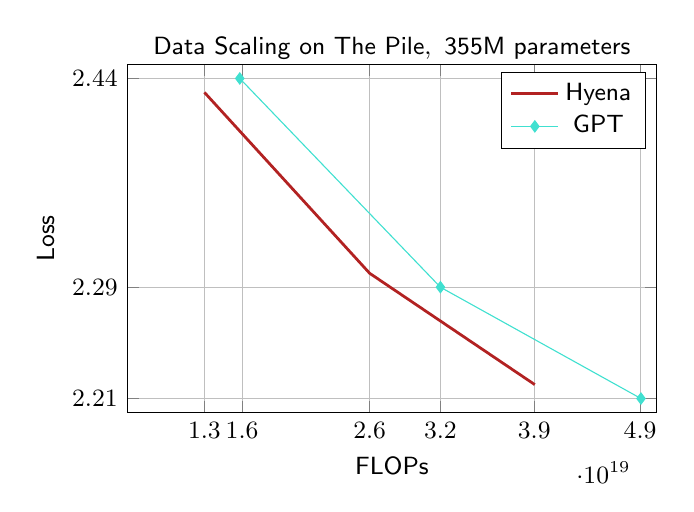
\begin{tikzpicture}[font=\small]

\definecolor{brown}{RGB}{165,42,42}
\definecolor{darkgray176}{RGB}{176,176,176}
\definecolor{firebrick}{RGB}{178,34,34}
\definecolor{indianred}{RGB}{205,92,92}
\definecolor{lightgray204}{RGB}{204,204,204}
\definecolor{lightseagreen}{RGB}{32,178,170}
\definecolor{teal}{RGB}{0,128,128}
\definecolor{turquoise}{RGB}{64,224,208}

\begin{axis}[
width=8.3cm, height=6cm,
title={$\small{{\sf Data~Scaling~on~The~Pile,~355M~parameters}}$},
title style = {at={(.5, .94)}},
xlabel={$\small \sf FLOPs$}, ylabel={$\small\sf Loss$}, 
ylabel style={at={(-.12,.5)}},
xmin=7e+18, xmax=4.9e+19, ymin=2.2, ymax=2.45,
major grid style={lightgray,thin},
minor grid style={lightgray,very thin},
grid=both,
%
xtick={1.311e+19,1.61e+19,2.623e+19,3.185e+19,3.93e+19,4.77e+19},
xticklabels={
  \(\displaystyle {1.3}\),
  \(\displaystyle {1.6}\),
  \(\displaystyle {2.6}\),
  \(\displaystyle {3.2}\),
  \(\displaystyle {3.9}\),
  \(\displaystyle {4.9}\)
},
ytick={2.44, 2.29, 2.21},
yticklabels={
  \(\displaystyle {2.44}\),
  \(\displaystyle {2.29}\),
  \(\displaystyle {2.21}\)
}
]
\addplot [mark=mystar, line width=1pt, firebrick]
table{%
x  y
1.311e+19 2.43
2.623e+19 2.30
3.934e+19 2.22
};\addlegendentry{$\sf Hyena$};
\addplot [draw=black, mark=diamond*, turquoise]
table{%
x  y
1.592e+19 2.44
3.185e+19 2.29
4.777e+19 2.21
};\addlegendentry{$\sf GPT$};
% \addplot [line width=1pt, indianred, opacity=0.4]
% table {%
% 3.227256e+18 17.01
% 6.454512e+18 14.16
% 9.681768e+18 12.58
% 1.2909024e+19 11.82
% 1.613628e+19 11.44
% };
% \addplot [line width=1pt, turquoise, opacity=0.4]
% table {%
% 4.12e+18 17.91
% 8.24e+18 14
% 1.236e+19 12.55
% 1.648e+19 11.76
% 2.06e+19 11.44
% };
% \addplot [line width=1pt, lightseagreen, opacity=0.4]
% table {%
% 4.12e+18 17.84
% 8.24e+18 13.92
% 1.236e+19 12.61
% 1.648e+19 11.62
% 2.06e+19 11.04
% 2.472e+19 10.59
% 2.884e+19 10.28
% 3.296e+19 10.04
% 3.708e+19 9.88
% 4.12e+19 9.79
% };
% \addplot [line width=1pt, teal, opacity=0.4]
% table {%
% 4.12e+18 17.76
% 8.24e+18 13.82
% 1.236e+19 12.43
% 1.648e+19 11.57
% 2.06e+19 11.04
% 2.472e+19 10.61
% 2.884e+19 10.27
% 3.296e+19 10.01
% 3.708e+19 9.79
% 4.12e+19 9.61
% 4.532e+19 9.55
% 4.944e+19 9.33
% 5.356e+19 9.23
% 5.768e+19 9.16
% 6.18e+19 9.12
% };
% \addplot [line width=1pt, brown, opacity=0.4]
% table {%
% 3.227256e+18 17.03
% 6.454512e+18 13.76
% 9.681768e+18 12.46
% 1.2909024e+19 11.67
% 1.613628e+19 11.2
% 1.9363536e+19 10.74
% 2.2590792e+19 10.37
% 2.5818048e+19 10.09
% 2.9045304e+19 9.9
% 3.227256e+19 9.8
% };
% \addplot [line width=1pt, firebrick, opacity=0.4]
% table {%
% 3.227256e+18 17.25
% 6.454512e+18 14.26
% 9.681768e+18 12.58
% 1.2909024e+19 11.95
% 1.613628e+19 11.46
% 1.9363536e+19 11.05
% 2.2590792e+19 10.72
% 2.5818048e+19 10.43
% 2.9045304e+19 10.18
% 3.227256e+19 9.97
% 3.5499816e+19 9.78
% 3.8727072e+19 9.62
% 4.1954328e+19 9.48
% 4.5181584e+19 9.35
% 4.840884e+19 9.24
% };
% % linear regressed values
% \addplot [line width=1pt, dotted, red, opacity=1]
% table {%
% 1.2e+19 11.54196759
% 7.2e+19 7.45180555
% };
% %
% \addplot [line width=1pt, dotted, blue, opacity=1]
% table {%
% 1.2e+19 11.76093851
% 7.2e+19 8.38229773
% };
\end{axis}

\end{tikzpicture}

    \vspace{-4mm}
    \caption{Preliminary "scaling law" of language models on {\sc The Pile}. Comparison of our approach (red) based on long convolutions and gating (${\sf Hyena}$) and a standard GPT (blue) \citep{brown2020language}. We reach perplexity of GPT with a smaller training FLOP budget.}
    \label{fig:hyena_laws}
\end{figure}


\begin{table}[t]
    \small
    \centering
    \begin{minipage}{.38\textwidth}
        \centering
        \caption{Perplexity on {\sc WikiText103} (same tokenizer). $^*$ are results from \citep{dao2022hungry}. Deeper and thinner models (Hyena-slim) achieve lower perplexity.}
        \vspace{2mm}
        \label{wt103}
        \setlength{\tabcolsep}{4pt}
        \begin{tabular}{@{}c|cc@{}}
        \toprule
        Model &\multicolumn{1}{c}{{\sc Perplexity}} \\
        \midrule 
        Transformer ($125$M) & $18.6$ & \\
        Hybrid H3 ($125$M) & $18.5^*$ \\
        Performer ($125$M) & $26.8^*$  \\ 
        Reformer  ($125$M)& $25.6^*$  \\ 
        \midrule
        AFT-conv ($125$M) & $28.2$ \\
        Linear Attention ($125$M) & $25.6^*$ \\
        \midrule
        ${\sf Hyena}$-$3$ ($125$M) & $18.6$ \\
        ${\sf Hyena}$-$3$-slim ($125$M) & $18.5$ \\
        \bottomrule
        \end{tabular}
    \end{minipage}
    %
    \hspace{0.7cm}
    %
    \begin{minipage}{.55\textwidth}
        \centering
        \vspace{-18mm}
        \caption{Perplexity on {\sc The Pile} for models trained until a total number of tokens e.g., $5$ billion (different runs for each token total). All models use the same tokenizer (GPT2). FLOP count is for the $15$ billion token run.}
        \vspace{2mm}
        \label{pile}
        \setlength{\tabcolsep}{4pt}
        \begin{tabular}{@{}c|cccc@{}}
        \toprule
        Model &\multicolumn{1}{c}{{\sc $5$B}} & \multicolumn{1}{c}{{\sc $10$B}} & \multicolumn{1}{c}{{\sc $15$B}} & \multicolumn{1}{c}{{\sc FLOPs ($10^{19}$)}}\\
        \midrule 
        GPT ($125$M) & $13.3$ & $11.9$ & $11.2$ & $1.88$ \\
        ${\sf Hyena}$-$2$ ($153$M)& $13.3$ & $11.8$ & $11.1$ & $\textbf{1.87}$ \\
        \midrule
        GPT ($355$M) & $11.4$ & $9.8$ & $9.1$ & $4.77$ \\
        ${\sf Hyena}$-$2$ ($355$M) & $11.3$ & $9.8$ & $9.2$ & $\textbf{3.93}$ \\
        \bottomrule
        \end{tabular}
    \end{minipage}
\end{table}

% \begin{minipage}{.5\textwidth}
%     \begin{table}[t]
%     \small
%     \centering
%     \caption{Perplexity on {\sc The Pile} for models trained until a total number of tokens e.g., $5$ billion (different runs for each token total, scheduler is adjusted). All models use the same tokenizer (GPT2). FLOP count is for the $15$ billion token run.}
%     \label{pile}
%     \setlength{\tabcolsep}{4pt}
%     \begin{tabular}{@{}c|cccc@{}}
%     \toprule
%     Model &\multicolumn{1}{c}{{\sc $5$B}} & \multicolumn{1}{c}{{\sc $10$B}} & \multicolumn{1}{c}{{\sc $15$B}} & \multicolumn{1}{c}{{\sc FLOPs ($10^{19}$)}}\\
%     \midrule 
%     GPT ($125$M) & $13.3$ & $11.9$ & $11.2$ & $1.88$ \\
%     ${\sf Hyena}$-$2$ ($153$M)& $13.3$ & $11.8$ & $11.1$ & $\textbf{1.87}$ \\
%     \midrule
%     GPT ($355$M) & $11.4$ & $9.8$ & $9.1$ & $4.77$ \\
%     ${\sf Hyena}$-$2$ ($355$M) & $11.3$ & $9.8$ & $9.2$ & $\textbf{3.93}$ \\
%     \bottomrule
%     \end{tabular}
%     \end{table}
% \end{minipage}

\subsection{Downstream Evaluation}
%
We perform a downstream evaluation on SuperGLUE \citep{wang2019superglue} tasks. We compare ${\sf Hyena}$ (trained for $137$ billion tokens) with the best available pre-trained attention-free model, RWKV \citep{PENG_RWKV-LM_2021} (trained for $332$ billion tokens), and a reference GPTNeo \citep{gpt-neo} (trained for $300$ billion tokens) of the same size. Tables \ref{supergluezero} and \ref{supergluefew} summarize the results. ${\sf Hyena}$ performs similarly to other models despite having been trained on less than half the number of total tokens. We observe ${\sf Hyena}$ to display characteristic few-shot capabilities of standard Transformers, with some tasks e.g., MultiRC seeing a lift of more than $20\%$ accuracy over zero-shot when the model is provided additional prompts as context. The improvements are more noticeable in generation tasks, where the additional prompts can instruct the model on how it should be responding to the questions. We report an additional downstream evaluation on the LAMBADA  task \citep{paperno2016lambada} in Appendix \ref{appendix:experiment-details}.
%
\begin{table}[!h]
\small
\centering
\caption{Zero-shot accuracy ($\%$) on {\sc SuperGLUE} tasks for small models.}
\label{supergluezero}
\vspace{2mm}
\setlength{\tabcolsep}{4pt}
\begin{tabular}{@{}c|ccccccccc@{}}
\toprule
Model &\multicolumn{1}{c}{{\sc WSC}} & \multicolumn{1}{c}{{\sc WIC}} & \multicolumn{1}{c}{{\sc RTE}} & \multicolumn{1}{c}{{\sc CB}} & \multicolumn{1}{c}{{\sc MultiRC}} &  \multicolumn{1}{c}{{\sc ReCoRD}} &  \multicolumn{1}{c}{{\sc BoolQ}} &  \multicolumn{1}{c}{{\sc COPA}} & \multicolumn{1}{c}{{\sc Average}} \\
\midrule 
GPTNeo \citep{gpt-neo} & $\mathbf{27.9}$ & $50.0$ & $45.1$ & $\mathbf{41.1}$ & $0.0$ & $\mathbf{61.7}$ & $\mathbf{62.2}$ & $62.0$ & $\mathbf{43.8}$ \\ 
RWKV \citep{PENG_RWKV-LM_2021} & $13.4$ & $\mathbf{52.3}$ & $\mathbf{46.9}$ & $25.0$ & $0.0$ & $58.5$ & $\underline{59.2}$ & $\underline{66.0}$ & $40.2$ \\
${\sf Hyena}$ & $\underline{21.2}$ & $\underline{50.5}$ & $\underline{46.6}$ & $\underline{39.3}$ & $\mathbf{1.1}$ & $\underline{59.4}$ & $51.8$ & $\mathbf{70.0}$ & $\underline{41.5}$ \\
\bottomrule
\end{tabular}
\end{table}
\begin{table}[!h]
\small
\centering
\caption{Few-shot ($3$) accuracy ($\%$) on {\sc SuperGLUE} tasks for small models.}
\label{supergluefew}
\vspace{2mm}
\setlength{\tabcolsep}{4pt}
\begin{tabular}{@{}c|ccccccccc@{}}
\toprule
Model &\multicolumn{1}{c}{{\sc WSC}} & \multicolumn{1}{c}{{\sc WIC}} & \multicolumn{1}{c}{{\sc RTE}} & \multicolumn{1}{c}{{\sc CB}} & \multicolumn{1}{c}{{\sc MultiRC}} &  \multicolumn{1}{c}{{\sc ReCoRD}} &  \multicolumn{1}{c}{{\sc BoolQ}} &  \multicolumn{1}{c}{{\sc COPA}} & \multicolumn{1}{c}{{\sc Average}} \\
\midrule 
GPTNeo \citep{gpt-neo} & $\underline{38.5}$ & $\underline{50.0}$ & $\mathbf{53.8}$ & $\underline{42.9}$ & $\underline{22.4}$ & $\mathbf{61.4}$ & $\mathbf{61.0}$ & $63.0$ & $\underline{49.1}$ \\ 
RWKV \citep{PENG_RWKV-LM_2021} & $32.7$ & $49.4$ & $47.2$ & $37.5$ & $0.0$ & $\underline{58.3}$ & $55.0$ & $\underline{64.0}$ & $43.0$ \\
${\sf Hyena}$ & $\mathbf{39.4}$ & $\mathbf{50.1}$ & $\underline{47.6}$ & $\mathbf{46.4}$ & $\mathbf{26.7}$ & $58.1$ & $\underline{56.0}$ & $\mathbf{70.0}$ & $\mathbf{49.3}$ \\
\bottomrule
\end{tabular}
\end{table}
%

%
\subsection{Benchmarking}
%
We benchmark runtime of an order $2$ ${\sf Hyena}$ operator compared to attention and FlashAttention layers \citep{dao2022flashattention}. ${\sf Hyena}$ uses a fused CUDA kernel to perform ${\sf FFTConv}$ \citep{dao2022hungry}. We set batch size to $64$ and measure runtime (in milliseconds). Results are provided in Figure \ref{fig:benchmarking_plot}. ${\sf Hyena}$ speedups reach $100\x$ at sequence length $64$K. Crossover points for ${\sf Hyena}$ and attention is at length $2048$, and for ${\sf Hyena}$ and FlashAttention is between $4096$ and $8196$. Despite the absolute reduction in FLOPs, speedups are achieved only on longer sequences when the gap grows sufficiently large. This occurs because hardware utilization of ${\sf Hyena}$ is lower than FlashAttention. We expect the gap between theoretical maximum speedup to shrink with improved implementations of ${\sf FFTConv}$ and specialized hardware.
%
\begin{figure}[t]
    \centering
    \begin{tikzpicture}[font=\footnotesize
]
\definecolor{brown}{RGB}{165,42,42}
\definecolor{cornflowerblue}{RGB}{100,149,237}
\definecolor{darkgray176}{RGB}{176,176,176}
\definecolor{indianred}{RGB}{205,92,92}
\definecolor{lightgray204}{RGB}{204,204,204}
\definecolor{teal}{RGB}{0,128,128}
\definecolor{lightseagreen}{RGB}{32,178,170}
 \begin{axis}[
   width=.5\linewidth, height=4cm,
   %scaled ticks=false,
   xmode=log,
   xmin=1000, xmax = 100000,
   ymin=0,
   xlabel=In,
   ylabel=out,
   name=ax1,
   xlabel={$\sf Sequence~Length$},
   ylabel={${\sf Runtime}~[ms]$},
 ]
\addplot [line width=1pt, indianred]
table {%
1024 0.9
2048 1.16
4096 1.47
8192 1.5
16384 2.84
32768 5.41
65536 11.32
};
\addplot [line width=1pt, cornflowerblue]
table {%
1024 0.4
2048 1.25
4096 2.16
8192 6.17
16384 21.74
32768 90.71
};
\addplot [line width=1pt, lightseagreen, dashed]
table {%
1024 0.29
2048 0.3
4096 0.63
8192 2.1
16384 8.33
32768 32.85
65536 129.07
};
 %\addplot[domain=15:140, blue, ultra line width=1pt,smooth] {f(x)};

  % define coordinates at bottom left and top left of rectangle
  \coordinate (c1) at (axis cs:1024,0);
  \coordinate (c2) at (axis cs:1024,7);
  % draw a rectangle
  \draw (c1) rectangle (axis cs:8196,7);


\end{axis}
%
\begin{axis}[
    width=.5\linewidth, height=4cm,
    name=ax2,
    xmin=1000,xmax=8192,
    ymin=0,ymax=7,
    xlabel={${\sf Sequence~Length}$},
    %ylabel=out,
    xmode=log,
    xminorgrids=true,
    legend style={font=\footnotesize, draw=none, fill=none, align=left},
    legend columns = 3,
    legend cell align={left},
    % place second axis relative to first one
    % anchor is south west
    at={($(ax1.south east)+(1cm,0)$)},
    % turn on grid
    % xmajorgrids=true,
    % grid style={help lines,dashed},
    % to avoid clipping of a...e nodes
    clip=false
 ]
    \addplot [line width=1pt, indianred, opacity=.9]
        table {%
        1024 0.9
        2048 1.16
        4096 1.47
        8192 1.5
    };\addlegendentry{$\sf Hyena$}
    \addplot [line width=1pt, cornflowerblue]
        table {%
        1024 0.4
        2048 1.25
        4096 2.16
        8192 6.17
    };\addlegendentry{$\sf Attention$}
    \addplot [line width=1pt, lightseagreen, dashed]
        table {%
        1024 0.29
        2048 0.3
        4096 0.63
        8192 2.1
    };\addlegendentry{$\sf FlashAttention$}
\end{axis}

% draw dashed lines from rectangle in first axis to corners of second
\draw [dashed] (c1) -- (ax2.south west);
\draw [dashed] (c2) -- (ax2.north west);

\draw ({$(current bounding box.south west)!0.5!(current bounding box.south east)$}|-{$(current bounding box.south west)!1.16!(current bounding box.north west)$}) node[
  scale=1,
  anchor=north,
  text=black,
  rotate=0.0
]{\textbf{Benchmarking~Hyena}};
\end{tikzpicture}
    \vspace{-5mm}
    \caption{Benchmarking runtime of Hyena, Attention and FlashAttention with varying sequence lengths. Batch size is set to $64$. The figure on the right is an inset showing a zoomed-in portion of the figure on the left.}
    \label{fig:benchmarking_plot}
\end{figure}

\subsection{Large-Scale Image Classification}\label{benchm}
\label{sec:image_classification}
Finally, we demonstrate the potential of ${\sf Hyena}$ as a general deep learning operator by applying it to image classification. On {\sf ImageNet}, we drop-in replace attention layers in the \textit{Vision Transformer} (ViT) \citep{dosovitskiy2020image} with the ${\sf Hyena}$ operator (without changes from its language counterpart) and match performance with ViT. We also show that using smaller image patches boosts performance in both attention and ${\sf Hyena}$. Since this results in longer sequence lengths, we expect ${\sf Hyena}$ to outperform in speed as patches get more fine-grained approaching pixel-level. On CIFAR-2D, we test a 2D version of ${\sf Hyena}$ long convolution filters in a standard convolutional architecture, which improves on the 2D long convolutional model S4ND \citep{nguyen2022s4nd} in accuracy with a $8\%$ speedup and 25\% fewer parameters. See Appendix \ref{appendix:image-classification} for additional vision architectures and training procedure details.

 %We show the potential of using smaller patch sizes (which increases the sequence length) to boost performance when using 8x8 patches (instead of 16x16)

\begin{table}[h]
\small
\centering
\caption{Image classification top-1 accuracy.}
\label{image_results}
\setlength{\tabcolsep}{4pt}
\begin{tabular}{@{}c|cccc@{}}
\toprule
Model & \multicolumn{1}{c} {{\sc Patch Size}} &  \multicolumn{1}{c} {{\sc Seq Len}} & \multicolumn{1}{c} {{\sc Dataset}} & \multicolumn{1}{c}{{\sc Acc (\%)}} \\
\midrule 
ViT ($87$M) & 16x16 & 196 & ImageNet-1k & 78.5 \\
Hyena-ViT ($88$M) & 16x16 & 196 & ImageNet-1k & 78.5 \\
\midrule
ViT ($87$M) & 8x8 & 1024 & ImageNet-1k & 80.0 \\
Hyena-ViT ($88$M) & 8x8 & 1024 & ImageNet-1k & 79.8 \\
\midrule
S4ND-ISO ($268$k) & - & - & CIFAR-10 & 89.9 \\
Hyena-ISO ($202$k) & - & - & CIFAR-10 & 91.2 \\
\bottomrule
\end{tabular}
\end{table}